\documentclass[11pt,english]{article}
\usepackage{lmodern}
\usepackage{amssymb,amsmath}
\usepackage{ifxetex,ifluatex}
\ifnum 0\ifxetex 1\fi\ifluatex 1\fi=0 % if pdftex
  \usepackage[T1]{fontenc}
  \usepackage[utf8]{inputenc}
\else % if luatex or xelatex
  \ifxetex
    \usepackage{mathspec}
  \else
    \usepackage{fontspec}
  \fi
  \defaultfontfeatures{Ligatures=TeX,Scale=MatchLowercase}
\fi
\usepackage[margin=1in]{geometry}
\usepackage{hyperref}
\hypersetup{unicode=true,
            pdftitle={Displacement of fishing effort by Large Scale Marine Protected Areas},
            pdfborder={0 0 0},
            breaklinks=true}
\urlstyle{same}  % don't use monospace font for urls
\usepackage{natbib}
\bibliographystyle{chicago}
\usepackage{longtable,booktabs}
\usepackage{graphicx,grffile}
\makeatletter
\def\maxwidth{\ifdim\Gin@nat@width>\linewidth\linewidth\else\Gin@nat@width\fi}
\def\maxheight{\ifdim\Gin@nat@height>\textheight\textheight\else\Gin@nat@height\fi}
\makeatother
% Scale images if necessary, so that they will not overflow the page
% margins by default, and it is still possible to overwrite the defaults
% using explicit options in \includegraphics[width, height, ...]{}
\setkeys{Gin}{width=\maxwidth,height=\maxheight,keepaspectratio}
\IfFileExists{parskip.sty}{%
\usepackage{parskip}
}{% else
\setlength{\parindent}{0pt}
\setlength{\parskip}{6pt plus 2pt minus 1pt}
}
\setlength{\emergencystretch}{3em}  % prevent overfull lines
\providecommand{\tightlist}{%
  \setlength{\itemsep}{0pt}\setlength{\parskip}{0pt}}
\setcounter{secnumdepth}{5}
% Redefines (sub)paragraphs to behave more like sections
\ifx\paragraph\undefined\else
\let\oldparagraph\paragraph
\renewcommand{\paragraph}[1]{\oldparagraph{#1}\mbox{}}
\fi
\ifx\subparagraph\undefined\else
\let\oldsubparagraph\subparagraph
\renewcommand{\subparagraph}[1]{\oldsubparagraph{#1}\mbox{}}
\fi

\title{Large Scale Marine Protected Areas}

\author{
  Juan CarlosVillase\~{n}or-Derbez\footnote{Bren School of Environmental Science \& Management, University of California at Santa Barbara, Santa Barbara, CA} \\
  \texttt{juancarlos@ucsb.edu}
  \and
 John Lynham\footnote{Department of Economics, University of Hawaii at Manoa, Honolulu, HI}\\
  \texttt{lynham@hawaii.edu }
}

\date{Updated on: \today}

\usepackage{float}
\floatplacement{figure}{H}
\usepackage{lineno}
\linenumbers
\usepackage[bottom]{footmisc}
\usepackage{pdflscape}
\newcommand{\beginsupplement}{\setcounter{table}{0}  \renewcommand{\thetable}{S\arabic{table}} \setcounter{figure}{0} \renewcommand{\thefigure}{S\arabic{figure}}}

% John's additional packages below

\usepackage{graphicx}
\graphicspath{{figures/}} %Setting the graphicspath

\begin{document}
\maketitle
\begin{abstract}
Large-scale Marine Protected Areas (LSMPAs) have seen a significant
increase over the last years. Fishing effort is effectively eliminated
within these protected areas upon implementation. The benefits of
reducing effort have been largely studied, but little empirical works
evaluate how vessels react and redistribute after an MPA is created. The
economic and ecological implications of displacing fishing effort are
not yet fully understood. We use identification of fishing activity via
Automatic Identification Systems (AIS) and causal inference techniques
to provide the first analysis of behavioral changes and spatial
redistribution of tuna purse seiners due to the implementation of a
Large Scale Marine Protected Area in the Pacific Ocean. Our work
provides three main findings: 1) aggregate fishing effort remains
relatively unaffected; 2) vessels that fished inside the protected area
redistribute to adjacent waters; and 3) we observe a crowding effect for
the first months after implementation. Our results not only provide an
impact evaluation of the effect of LSMPAs on fishing activity, but
provide insights into vessel redistribution dynamics, which may have
ecological and economic implications for marine conservation and fisheries
management. As countries continue to implement LSMPAs as a way to
reach the stated 10\% target of ocean protection, managers should
consider how fishing effort will change in space and through time to
ensure that fishing effort is not just displaced elsewhere, leading to
overfishing in adjacent waters. While LSMPAs can provide a wide
range of benefits, their implementation must be accompained with
traditional fisheries management to maximize their effectiveness.


We do not observe an increase in daily fishing hours for vessels that used to fish within PIPA, compared to a control
group of vessels. Thus, for vessels that have chosen to continue to operate following the closure, we do not observe evidence that they are being forced to exert more effort as a result of the closure. Unfortunately, without detailed data on vessel catch, we cannot conclude whether vessels are better or worse off financially following the closure.

Our results suggest that PIPA has displaced some vessels to the high seas just outside the EEZ of Kiribati. This might imply a drop in demand for Kiribati fishing rights and a decline in revenue. We also uncover evidence that there is more congestion immediately following the closure, but this is declining over time.
\end{abstract}

\clearpage

Next steps: I think we need to make the buffers around the EEZs 5 degrees instead of 1 degree (redistribution of effort section)
Might change the specification of the redistribution regression


\section{Introduction}\label{introduction}



Marine Protected Areas (MPAs) are intended to safeguard parts of the
ocean from fishing and other extractive activities. Current
international goals aim to protect 10\% of the ocean environment by
2020. In an effort to meet this target, there has been a rapid
increase recently in MPA coverage \citep{wood_2008,sala_2018}, largely driven by
a small number of Large Scale Marine Protected Areas (LSMPAs).\footnote{See, for example, \citet{game_2009},  \citet{singleton_2014},\citet{boonzaier_2016}, \citet{mccauley_2016}, and \citet{alger_2017}.}
). Today, a small number of LSMPAs make up at least 80\%
of the managed areas in the ocean \citep{toonen_2013}.

Given the relatively recent establishment of most LSMPAs, very little is
known about their human dimensions and implication for fisheries
\citep{gray_2017}. As with smaller MPAs, it is important that we
understand the socioeconomic implications of management interventions.
One issue of particular importance is that of the displacement or
redistribution of fishing effort, which may influence the outcomes of an
MPA \citep{smith_2003}. Theoretical models make different assumptions
about the ways in which fishers will reallocate fishing effort after an
area closure, which often determine whether or not MPAs produce negative or positive impacts on fisheries. The existing empirical literature focuses on small MPAs and has been criticized for confounding correlation with causation \citep{ferraro2018causal}.

Recent advances in satellite tracking technologies and near real-time
identification of fishing activity provide us with an opportunity to ask, how do fishers respond to the implementation of an LSMPA? Does effort increase or decrease and where does it go? We use identification of fishing activity via Automatic
Identification Systems (AIS) and causal inference techniques to describe
the behavioral changes and spatial redistribution of the industrial tuna
purse seine fleet due to the implementation of the Phoenix Islands Protected Area. We use the same data to hypothesize what might be the impacts of the proposed Palau National Marine Sanctuary.

Our work is novel in the sense that it provides empirical evidence of
the effect of Large Scale Marine Protected Areas on fishing behavior and
distribution and can help guide future interventions. Understanding how
effort is displaced from LSMPAs might provide insights into how distant water fishing fleets would react to a high seas closure.

The paper is organized as follows: Section \ref{background} provides more
information on Large Scale Marine Protected Areas and some background on
empirical studies of effort redistribution. An overview of the Nauru
Agreement and associated countries, a description of the fleet that
operates in the region, and a brief history of PIPA and PNMS is also included.
Section \ref{methods} describes our data and identification strategy.
Section \ref{results} presents our results, and Section \ref{discussion}
discusses our
results.

\section{Background}\label{background}

\hypertarget{large-scale-marine-protected-areas}{%
\subsection{Large Scale Marine Protected
Areas}\label{large-scale-marine-protected-areas}}

The cutoff at which an MPA is considered to be a LSMPA ranges from areas
larger than 30,000 km\textsuperscript{2} as defined by
\citet{desanto_2013} or areas larger than 250,000 km\textsuperscript{2},
as defined by \citep{toonen_2013}. Figure \ref{fig:LSMPAs_map} shows
LSMPAs that meet the latter condition, and are also fully no-take. LSMPAs are often
implemented in the pelagic environment, where the dominant human
activity is industrial fishing \citep{gray_2017,kroodsma_2018}. The
early literature on LSMPAs focused on the inherent challenges and
difficulties that come with a pelagic environment. \citet{kaplan_2010}
claimed that very large MPAs would result in excessive opportunity costs
and that these would be difficult to enforce. \citet{game_2009}
suggested that most of the challenges could be overcome with the
incorporation of technology, in what then became known as Dynamic Ocean
Management \citep{maxwell_2015}.\footnote{See \citet{singleton_2014}, who provide an objective discussion of the pros and cons of LSMPAs.} 

\begin{figure}
\centering
\includegraphics{img/LSMPAs_map.pdf}
\caption{\label{fig:LSMPAs_map}Large Scale Marine
Protected Areas. The map shows all areas larger than 250,000
Km\textsuperscript{2}. Areas in dark blue meet at least one of these
conditions: reported no take area is greater than 0, are categorized as
IUCN Ia or Ib, their designated English name is `Protected Area'.}
\end{figure}

LSMPAs were erroneously assumed to have little social implications due
to their remoteness. However, there have been calls to incorporate the
human dimensions into LSMPAs management and evaluation
\citep{agardy_2011,gray_2017}. Most research incorporating these
dimensions has focused on governance and enforcement of LSMPAs
(\emph{i.e.} \citet{alger_2017,christie_2017}), but they are yet to be
the focus of economic analyses \citep{gray_2017}. Overall, there has
been little empirical work regarding LSMPAs. Recent technological
advances in vessel-detection systems allows for the discovery and
advancement of many important facets of LSMPAs. For example,
\citet{mcdermott_2018} show that the anticipation of a LSMPA can lead to
preemptive overfishing, which can erode or delay the expected benefits
of the intervention. \citet{white_2017} combine shark tags and
vessel-tracking data to demonstrate that the fairly large Palmyra Atoll
National Wildlife Refuge (54,000 Km\textsuperscript{2}) protects two
thirds of the tagged grey reef sharks by effectively excluding fishing
effort. More recently, \citep{bradley_2018} use similar data to
highlight cases of potential illegal shark fishing \emph{inside} a 2
million km\textsuperscript{2} shark sanctuary. To date, no studies have
evaluated the displacement of fishing effort due to LSMPA
implementation.

Spatial closures of this magnitude are likely to induce changes in
fishers' behavior. Theoretical models of fishing effort redistribution
range from the simplistic assumption that effort inside the bounded
region disappears, to spatially explicit models that reallocate fishing
effort based on habitat characteristics, presence of other vessels, and
expected returns \citep{smith_2003,hilborn_2006}. However, these focus
on the long term optimal equilibrium, and redistribution of fishing
effort may not always be optimal, especially over the first few years
\citep{stevenson_2013}.

The empirical research that has been done in smaller sized MPAs
suggests that resource users may show idiosyncratic responses. For
example, \citet{stevenson_2013} show that a network of MPAs displaced
fishing effort farther away from ports, resulting in higher
\emph{perceived} costs, and increases in catch per unit effort.
\citet{cabral_2017} analyze the redistribution of fishing and
non-fishing vessels following the implementation of a network of MPAs in
California, and find that commercial dive boats (??????) follow a
fishing-the-line pattern, while some fishing boats follow an ideal free
distribution. More recently \citet{elahi_2018} used satellite tracking
data to show that a temporal spatial closure caused trawlers to maintain
effort but apply it more intensively elsewhere, particularly along the
borders and closer to shore. The way in which fishers react to a spatial
closure can have major implications for its outcome
\citep{smith_2003,hilborn_2006}, highlighting the need to understand how
fishers react to the implementation of LSMPAs, how fishing effort
changes, and how it is spatially redistributed. All these closures took
place within Exclusive Economic Zones, where other regulations exist.
This may not always be the case for LSMPAs, where often the entire EEZ
is converted into a LSMPA, leaving fishers with the option of moving to
the high seas or other countries' EEZs.

\hypertarget{nauru-agreement-and-the-phoenix-island-protected-area}{%
\subsection{Nauru agreement and the Phoenix Islands Protected
Area}\label{nauru-agreement-and-the-phoenix-island-protected-area}}

The Nauru Agreement was established in 1982 by a select group of Pacific
island nations to manage their important tuna resources more effectively. Parties to the Nauru Agreement (PNA) Members
include the Federated States of Micronesia, Kiribati, the Marshall Islands,
Nauru, Palau, Papua New Guinea, the Solomon Islands, and Tuvalu. The Nauru
Agreement regulated access of foreign vessels (\emph{i.e.} those from
non-PNA countries). Holding \textasciitilde{}80\% of the historical
purse seining grounds within their Exclusive Economic Zones, PNA
countries gained greater bargaining power when providing fishing access to foreign
fleets \citep{havice_2010}.

The cooperation that emerged under the Nauru Agreement allowed for subsequent
agreements that strengthened fisheries management, like the Palau
Agreement, which limited the number of purse seiners at 205 vessels from
1995-2007\footnote{See \citet{havice_2010} for a detailed description of
  the Nauru, Palau, and Federal States of Micronesia agreements.}. However, the most notable regulation is
their approach to manage fishing effort: a Vessel Day Scheme (VDS)
implemented in 2007 \citep{havice_2013}. This effectively modified how
fishing effort was managed, from number of vessels under the Palau
Agreement to fishing hours. The VDS works as follows: Each year,
scientific advisers recommend a total number of fishing vessel-days per
year. Hours are allocated to each PNA country based on catch history,
and they then use or sell fishing rights to other non-PNA countries
\citep{aqorau_2018}. While the effectiveness of this scheme has been
debated in terms of meeting their fishery management and conservation
objectives, the licensing significantly contributes to the economy of
these island nations \citep{havice_2010}.

\begin{figure}
\centering
\includegraphics{img/PNA_map.pdf}
\caption{\label{fig:PNA_map}Map of the Exclusive
Economic Zones (EEZs) of the region of interest. Countries that belong
to the PNA are shown in blue, while empty polygons indicates all others.
A red line indicates the Kiribati EEZ, and a solid red polygon
delineates PIPA.}
\end{figure}

The main tuna species caught in the region are skipjack
(\emph{Katsuwonus pelamis}), yellowfin (\emph{Thunnus albacares}),
albacore (\emph{Thunnus alalunga}) and bigeye (\emph{Thunnus obesus}).
From these, the first two are amongst the top-10 species represented in
global fisheries production statistics, with 2016 catches increasing
relative to the 2005-2014 average \citep{fao_2018}. This region of the
Pacific has historically accounted for a large portion of tuna catches
\citep{aqorau_1997}. Today, the PNA controls close to 50\% of the global
skipjack tuna production \citep{pna_website_2018}. A large portion of
these catches derive from purse seine vessels licensed under the VDS.
Fishing vessels from Australia, New Zealand, China, France, Korea,
Japan, the Philippines, Taiwan, and the United States participate in the
purse-seining VDS.

One of the most notable and recent management interventions in the
region is the implementation of the Phoenix Islands Protected Area (PIPA)
by the government of Kiribati. PIPA was first declared in 2006, and
established in 2008 with only 4\% of the area declared as no-take. On
January 1\textsuperscript{st}, 2015, the no-take area within PIPA was
expanded to a total area of 397,447 km\textsuperscript{2}, roughly 1.5
times the size of Ecuador. Figure \ref{fig:PNA_map} shows a map of the
PNA countries and the Phoenix Islands Protected Area.

The closure of such a large area in one of the most important fishing
regions in the world provides a unique opportunity to evaluate the
behavioral responses and redistribution of fishing effort by vessels
that used to fish there. PIPA has been the focus of previous research
showing that fishing effort is effectively reduced after implementation
\citep{mccauley_2016,mcdermott_2018}. To this, we pose two questions:
How did individual vessels respond to the sudden exclusion of such a big
area? Where did all the vessels go? And what does this imply for revenues from
selling VDS for both Kiribati and the PNA as a whole? 

A spatial closure might cause fishers to modify
their behavior as they adapt to a new state of the world. For example, some may have
to travel further distances to find new fishing grounds, increasing their fuel
costs. If fishers had developed experience for fishing in particular
sites, being excluded might impose a learning cost on them, as they
identify new fishing grounds. This might result in increased search
times. However, if the area of knowledge of a vessel is significantly
larger than that of the spatial closure, they might already know other
places to fish. In the next sections we describe
the data and methods used to answer these questions.

\section{Methods}\label{methods}

This section is divided into two main parts. First, we provide a general
description of AIS data and the process of identification of
vessel-level fishing events performed by Global Fishing Watch.\footnote{Global Fishing Watch: \url{globalfishingwatch.org}}
Alongside, we describe
the subset of data used in our analysis. We also point
out possible shortcomings in the data, or factors that must be
considered in the analysis. We then move on to explain our
empirical strategy for the identification of behavioral changes and
the redistribution of fishing effort.

\subsection{Data}\label{data}

Automatic Identification Systems (AIS) are on-board devices that provide
at-sea safety and prevent ship collisions by broadcasting vessel
position, course, and activity to surrounding vessels. These broadcast
messages can be received by satellites and land-based antennas. GFW then uses 
machine learning techniques (convolutional neural networks) on the broadcast messages
to infer what type of fishing is taking place and where it is taking place, thus
allowing the estimation of near real-time fishing events globally \citep{kroodsma_2018}.

The amount of data gathered by GFW is dependent on the number of antennas and
satellites that can receive signals. The total satellite count increased from 3 to 6 on 
June 1\textsuperscript{st}
2014 , and then from 6 to 10 on January
1\textsuperscript{st} 2016. This causes an increase in the number of
\emph{received} AIS messages (\emph{i.e.} points), and therefore an
apparent increase in the number of vessels and fishing hours. However,
the addition of new satellites affects all vessels in the same way. 

Our analysis focuses on purse seine vessels, the most important fishery
for PNA
countries.\footnote{We perform some of the same analyses for longliners and include them in the Appendix}
We identify a total of 103 purse seiners that fished in PNA waters at
least once before
2015\footnote{New vessels that entered the fishery after 2015 were not exposed to the policy intervention in the pre-treatment period and are therefore excluded from our analyses.}.
These vessels represent over 26 million individual observations for the
2012 - 2017 period. We identify 65 vessels that have fished inside PIPA
at least once since 2012. From these, 62 did so before the announcement
(\emph{i.e.} 09/01/2014 \emph{sensu} \citep{mcdermott_2018}) but we are
only able to track 61 for the complete period of study before and after
its
implementation.\footnote{1 vessel never fished again after August 18, 2013.}
On the other hand, 38 vessels never fished inside PIPA but we only have
data for 26 of these vessels both before and after MPA implementation.

Therefore, our treatment group contains all purse seiners (n = 61) that
fished within PIPA at least once before the announcement, and that
continued to fish elsewhere after the January 2015 implementation.
Vessels in the control group meet the following two conditions: i)
never fished within PIPA waters from 2012-2015, and ii) vessels have fished in
surrounding areas (\emph{i.e.} PNA-countries' EEZ) before and after PIPA
closure (n = 26).

We include three additional control groups as a
robustness check. The first group contains only vessels that belong to PNA countries (n
= 7). The second group excludes Chinese vessels (n = 21). Our third control
is made up of Japanese purse seiners that fish in the Pacific but have
never fished inside PIPA (n =
27).\footnote{We also considered a control group of Taiwanese flagged vessels but there are only 4 vessels with pre-2015 data.}
Our main definition of treatment and control groups leaves us with 61 treated and 26
control vessels, which have just over 22 million
observations with about 22\% of these observations identified as fishing events by the neural network classification.

For each vessel, we calculate total daily fishing hours and build a daily panel
with 37,800 observations. Table \ref{tab:baci_n_s} shows the number
of vessels following a Before-After-Control-Impact (BACI) design, as well as the fishing hours, before
and after PIPA. Fig. \ref{fig:all_panels} shows that mean fishing hours
for purse seiners have an abrupt increase, just before January 1st,
2015. This trend is observed for both treated and control groups. Across
all measures, the treatment and control vessels follow similar patterns,
confirming our claim that the control group provides a plausible
counterfactual. Figure \ref{fig:baci_strict} in the Appendix provides a visual
representation of the vessel-level fishing events that make up each
group through time. We use this panel data to answer our key research questions: 
Are the 61 purse seiners that used to fish within PIPA affected by the closure? If so, how?
What are they doing differently and where are they going that they didn't go to before?
The following section describes our empirical identification strategy.

\begin{table}[H]

\caption{\label{tab:}\label{tab:baci_n_s}Number of fishing vessels and mean daily fishing hours by group before and after PIPA implementation.}
\centering
\begin{tabular}[t]{lrrrr}
\toprule
Group & n & Before & After & Change (A / B)\\
\midrule
Control & 28 & 7.15 & 10.68 & 1.49\\
Treatment & 64 & 6.21 & 9.89 & 1.59\\
\bottomrule
\end{tabular}
\end{table}

\subsection{Analyses}\label{analyses}

Our first analysis focuses on identifying the response of 
vessels to the PIPA closure. We use daily fishing hours, daily proportion of fishing vs.~non-fishing
hours, daily distance traveled (km), distance from shore (km) and
distance from home
port(km) as our main outcomes of interest.
We compare these outcomes before and after the implementation
of PIPA using a Difference-in-Differences approach. Our main
specification is the following:

\[
y_{i,t} = \alpha + \beta_1 Post_t + \beta_2 Treat_i + \beta_3 Post_t \times Treat_i + \phi_t + \gamma_i + \theta_t + \epsilon_{i,t},
\]

where \(y_{i,t}\) is the outcome of interest for vessel \(i\) on day \(t\). A dummy variable \(Post_t\) takes the value of 0 for all
dates prior to PIPA implementation and a value of 1 for all dates
following PIPA implementation. \(Treat_i\) is a dummy
variable indicating whether a vessel belongs to the treatment (\(Treat_i = 1\)) or control
(\(Treat_i = 0\)) group. \(\alpha\) is
the standard intercept term, \(\beta_1\) captures the temporal trend,
\(\beta_2\) captures the initial difference between treated and control groups,
and \(\beta_3\) is our parameter of interest: the Difference-in-Differences estimate capturing
the treatment effect. Finally, \(\phi_t\) and \(\gamma_i\) represent
month and flag dummies that account for seasonality or
country-level management interventions. \(\theta_t\) are time dummies to
account for the addition of more satellites over time.\footnote{We test for other more complex specifications that interact a quarterly dummy or year-month dummies with the treatment group and find qualitatively the same results.}

Our second part of the analysis focuses on the redistribution of fishing
effort. The role of institutions may play an important role. As stated
before, LSMPAs often span the entirety of an EEZ. In the case of purse
seining in the PNA, vessels purchase access to the fishery at the
beginning of the season (QUESTION FOR JC: WHEN IS THIS? And wasn't the closure expected?). If a vessel decides to fish within the PNA,
they've already made the decision to pay for access, expecting higher
returns from fishing there than in the high seas. In the particular case
of PIPA, one would expect that a vessel previously holding a permit to fish in
Kiribati waters would 
most likely continue to purchase access to PNA waters (either in Kiribati's remaining open areas or a nearby EEZ). Alternatively, if a vessel fishes illegally
in Kiribati waters before the implementation, one would expect them to
reallocate to other regions with equal or less enforcement. In this
case, they might then choose to move to other Kiribati waters, waters
of countries that have similar enforcement levels, or to the high seas.

We discretize spatial units by creating a polygon for
PIPA and distinct
spatial units for each geographically separate EEZ of each country. Some vessels might shift
from EEZs into the high seas, but we are interested in knowing
\emph{where} in the high seas, so we incorporate additional regions by
using a 1 degree buffer of the high seas around each of the EEZ regions.
The rest of the high seas are merged into a single spatial unit. For
example, if we were to do this only for Kiribati, we would have 8
spatial units: PIPA, three EEZ units, three 1-degree buffers of high seas
around each EEZ, and the rest of the high seas. Whenever the buffer units
overlap, we randomly clip one on to the other (QUESTION FOR JC: WHAT DOES THIS MEAN?).

We then take these spatial polygons and rasterize them to a 1-degree grid
(see Figure \ref{fig:raster_rgn} in the Appendix), which we then use to rasterize points
of fishing activity. For each cell, we calculate the total monthly
fishing hours by treated and control vessels (see Figure
\ref{fig:fishing_raster}). Since we are interested in the redistribution
of fishing effort, we use this gridded data to calculate the proportion
of fishing hours that each region receives each month relative to the
total fishing hours observed across all regions and all cells in that
month.

We use this measure to evaluate the change in effort allocation by
regressing it on the interaction between a year dummy and a dummy for
regions:

\[
y_{i,t} = \alpha + \beta_1Year_t + \beta_{2,i}Region_i + \beta_{3,i}Year_t \times Region_i+ \epsilon_{i,t}
\]

Our variable of interest, \(y_{i,t}\) represents the proportion of
fishing hours that region \(i\) receives at time \(t\). Years are
modeled as factors (\(Year_t\)), using 2012 as the reference level.
\(Region\) is a dummy variable for regions defined above. Our parameter (QUESTION FOR JC: VECTOR?)
of interest is \(\beta_{3,i}\), which captures the yearly by-country
change in proportional allocation of fishing effort relative to 2012.

All regression coefficients were estimated via ordinary least squares,
and heteroskedasticity-robust standard errors were calculated. All analyses
were performed in R version 3.5.1 \citep{rcore_2018}. Raw data and code
used in this work are available on
\href{https://github.com/jcvdav/MPA_displacement}{github}.

\section{Results}\label{results}

Regression coefficients for our DiD analysis are shown in Table
\ref{tab:did}. Columns 1 -3 use our primary control group. Columns 4 - 6 use
only PNA vessels as controls, and columns 7 - 9 exclude Chinese vessels.
Columns 10 and 11 use Japanese vessels in the Pacific as controls, and
don't include flag fixed-effects to avoid perfect collinearity
between the Japanese flag and
control group status.
Our DiD analysis shows an overall increase in purse seine fishing hours,
even after accounting for the introduction of new satellites (Table
\ref{tab:did}).\footnote{Results of the same analysis is shown for longliners in Table \ref{tab:long}} This 
\emph{post} coefficient estimate is consistent across different
model specifications and across controls, and
effectively represents the patterns observed in Figure
\ref{fig:all_panels}.

The \(\beta_3\) coefficient indicating our treatment effect suggests
that, relative to the control, treated vessels fish less: to the order
of 0.5-3.7 hours per day. In 6 out of 11 specifications, there is a statistically significant decrease in daily fishing hours. Another way to interpret this is that the increase
in fishing effort by treated vessels has occurred at a lower rate than
control vessels. These values are equivalent to a reduction of 15 - 111 fishing hours per month. However, this result is only robust and
significant (\(p < 0.01\)) in the simplest specification of the
Diff-in-Diff. When reducing the linear structure of the
\(Pre \times Post\) design and instead interacting the treatment dummy
with quarterly or year-month combinations, we are not able to reject the
null hypothesis of no change, suggesting that the total fishing hours
remains similar for the displaced vessels (Figs.
\ref{fig:q1}-\ref{fig:ym4}). Since vessels don't seem to be fishing a lot less, an obvious question arises: where are they
fishing now?

Figure \ref{fig:fishing_raster} provides a spatial representation of
these changes. Note that the 2013 effort distribution is roughly similar
across vessels. Then, in 2014, there is a sharp increase in fishing hours
by treated vessels inside PIPA (the so-called Blue Paradox). In 2015, treated vessels
then allocate more effort to the easternmost Kiribati EEZ and the high seas. In 2016, the spatial distribution of
fishing effort is again similar across groups. It is evident that the
increase in relative fishing effort is greater for regions closer to
PIPA.

Along a similar line, Figure \ref{fig:redist_trend} shows a detailed
temporal evolution of the relative allocation of fishing
effort.\footnote{Recall that to evaluate the redistribution of fishing effort we only track fishing vessels that belong to the treated group.}
It shows the change in fishing effort inside PIPA, including the
preemptive fishing and immediate reduction previously reported
\citep{mcdermott_2018}. Kiribati waters in KIR 1 and KIR 2 show an
increase in fishing effort for 2015; the same pattern is observed for
their respective High Seas buffers, and the general High Seas. Other
regions farther away from PIPA don't show a clear pattern under visual
inspection. This suggests fishing effort inside PIPA has moved to the high seas around Kiribati instead of paying to fish within alternative Kiribati EEZ waters.

We then move on to our regression results, presented as a figure showing
the year-region interaction coefficient estimates for each region as a
stream of changes through time (Figure \ref{fig:mean_change} and Table
\ref{tab:mean_change}). As noted before, the marginal change in the
relative allocation of fishing effort relative to 2012 increases in 2014
for PIPA. Most coefficients are not statistically significant, but
follow the same trends previously discussed, with a tendency for regions
closer to PIPA to show an increase in the relative allocation of fishing
effort in the post-implementation period. The largest increase is
observed for the Kiribati EEZ 2, where the redistribution of treated
vessels caused a 15\% increase in the \emph{relative} allocation of
fishing effort within Kiribati waters. This displacement is likely
causing a crowding effect after PIPA-fishing vessels redistribute to
other areas.

We use the rasterized effort to evaluate if the PIPA closure increased
crowding outside the LSMPA. We count the number of raster cells that
had both treated and control vessels each year (Fig.
\ref{fig:sp_corr}A). The pattern observed here could just be an artifact
of satellite detections increasing though time. Therefore we also
calculate a spatial correlation of presence/absence and observe similar
patterns (Fig. \ref{fig:sp_corr}B). While this is at the year level and
cannot assure that vessels were in effect at the same time in the same
place, it provides a of what we would expect to
find if our claims of displacement are true. Spatial overlap increases
in 2015 as vessels from PIPA are excluded, but then starts to decline. [QUESTIONS FOR JC: Is this significant? Can we do a daily measure? What about mean or shortest distance between vessels. Treated/Control/Combined]

\begin{figure}
\centering
\includegraphics{img/all_panels.pdf}
\caption{\label{fig:all_panels}Time seri showing mean monthly values es for our 10 variables of interest:
A) Fishing hours, B)Non-fishing hours at-sea,
C) Proportion of fishing hours to total hours at-sea,
D) Distance traveled, E) Mean distance from port,
F) Mean distance from shore,
G) Mean distance from port for fishing events,
H) Mean distance from shore for fishing events,
I) Proportion of hours spent in Kiribati waters,
J) Proportion of fishing hours spent in PNA waters.}
\end{figure}

\clearpage
\begin{landscape}



\begin{table}[!htbp] \centering 
  \caption{\label{tab:main_DID}Difference-in-differences estimates for our 10 variables of interest: 1) Daily fishing hours, 2) Daily non-fishing at-sea hours, 3) Daily proportion of fishing hours to total at-sea hours, 4) Daily distance traveled, 5) Daily mean distance from port for fishing events, 6) Daily mean distance from shore for fishing events, 7) Monthly fishing hours spent in Kiribati waters, 8) Monthly fishing hours spent in PNA waters, and 9) Monthly fishing hours in the high seas. Numbers in parentheses are heteroskedastic-robust standard errors.} 
  \label{} 
\footnotesize 
\begin{tabular}{@{\extracolsep{1pt}}lccccccccc} 
\\[-1.8ex]\hline 
\hline \\[-1.8ex] 
\\[-1.8ex] & (1) & (2) & (3) & (4) & (5) & (6) & (7) & (8) & (9)\\ 
\hline \\[-1.8ex] 
 Constant & 0.497$^{***}$ & 3.607$^{***}$ & 0.075$^{***}$ & 5.203$^{***}$ & 12.997$^{***}$ & 12.461$^{***}$ & 3.678$^{***}$ & 4.445$^{***}$ & 2.420$^{***}$ \\ 
  & (0.022) & (0.012) & (0.004) & (0.029) & (0.021) & (0.019) & (0.192) & (0.151) & (0.421) \\ 
  & & & & & & & & & \\ 
 Post & 0.839$^{***}$ & $-$0.228$^{***}$ & 0.137$^{***}$ & 0.304$^{***}$ & 0.326$^{***}$ & 0.296$^{***}$ & 1.059$^{***}$ & 1.180$^{***}$ & 0.920$^{***}$ \\ 
  & (0.016) & (0.008) & (0.003) & (0.019) & (0.014) & (0.014) & (0.140) & (0.109) & (0.273) \\ 
  & & & & & & & & & \\ 
 Treated & 0.136$^{***}$ & 0.014$^{**}$ & 0.015$^{***}$ & 0.400$^{***}$ & 0.223$^{***}$ & 0.116$^{***}$ & 0.534$^{***}$ & 0.149 & $-$0.244 \\ 
  & (0.013) & (0.007) & (0.002) & (0.020) & (0.016) & (0.016) & (0.148) & (0.118) & (0.236) \\ 
  & & & & & & & & & \\ 
 Post $\times$ Treated & $-$0.244$^{***}$ & 0.013 & $-$0.034$^{***}$ & $-$0.483$^{***}$ & $-$0.281$^{***}$ & $-$0.155$^{***}$ & $-$0.565$^{***}$ & $-$0.399$^{***}$ & 0.338 \\ 
  & (0.019) & (0.009) & (0.003) & (0.022) & (0.017) & (0.017) & (0.161) & (0.127) & (0.288) \\ 
  & & & & & & & & & \\ 
\hline \\[-1.8ex] 
Month FE & Yes & Yes & Yes & Yes & Yes & Yes & Yes & Yes & Yes \\ 
Flag FE & Yes & Yes & Yes & Yes & Yes & Yes & Yes & Yes & Yes \\ 
Observations & 83,052 & 83,052 & 83,051 & 64,387 & 32,055 & 32,055 & 1,814 & 2,588 & 684 \\ 
R$^{2}$ & 0.102 & 0.072 & 0.107 & 0.028 & 0.062 & 0.080 & 0.113 & 0.198 & 0.233 \\ 
\hline 
\hline \\[-1.8ex] 
\textit{Note:}  & \multicolumn{9}{r}{$^{*}$p$<$0.1; $^{**}$p$<$0.05; $^{***}$p$<$0.01} \\ 
\end{tabular} 
\end{table} 


\end{landscape}
\clearpage

\begin{figure}
\centering
\includegraphics{img/other_specifications.pdf}
\caption{\label{fig:other_specifications}Alternative difference-in-differences estimates
for our variables of interest using different model specifications. Table \ref{tab:main_DID}
reports estimates for models with month and flag fixed effects (\emph{i.e.} green dots).}
\end{figure}

\begin{figure}
\centering
\includegraphics{img/fishing_raster.png}
\caption{\label{fig:fishing_raster}Yearly
spatial distribution of fishing effort by treated and control vessels.
Color corresponds to \% of total fishing effort in each panel.
Red polygons show LSMPAs in the region.}
\end{figure}

\begin{figure}
\centering
\includegraphics{img/redist_trend.pdf}
\caption{\label{fig:redist_trend}Monthly
relative allocation of fishing effort by PIPA-fishing vessels before and
after PIPA by region. Colors indicate the pre- and post- periods. Solid line
across points shows local mean with a region-specific loess smoother.
Vertical dashed lines indicates dates when satellites were added, solid vertical
line indicates PIPA closure. Note that inflection points of
the loess smoother are not affected by the addition of satellites.}
\end{figure}

\begin{figure}
\centering
\includegraphics{img/mean_change.pdf}
\caption{\label{fig:mean_change}Coefficient
estimates for the redistribution regression. Each panel shows the
region-specific coefficients, with 95\% condifence intervals
as error bars. The horizontal dashed line represents 0 change
relative to the 2012 region-specific levels.}
\end{figure}

\clearpage
\begin{landscape}

\begin{table}

\caption{\label{tab:mean_change}Coefficient estimates for the interaction of year and region. Each row represents a region, each color a year. Numbers in parentheses are heteroskedatic-robust standard errors.}
\centering
\begin{tabular}[t]{llllll}
\hline
\hline 
Coefficient & 2013 & 2014 & 2015 & 2016 & 2017\\
\hline
PIPA PIPA 1 & -0.047 (0.022)** & 0.106 (0.042)** & -0.072 (0.021)*** & -0.068 (0.021)*** & -0.075 (0.022)***\\
EEZ KIR 1 & -0.039 (0.034) & 0.030 (0.043) & 0.040 (0.045) & -0.046 (0.034) & -0.043 (0.037)\\
EEZ KIR 2 & 0.003 (0.010) & 0.028 (0.019) & 0.101 (0.045)** & 0.019 (0.018) & -0.004 (0.015)\\
EEZ KIR 3 & -0.199 (0.071)*** & -0.067 (0.072) & -0.111 (0.065)* & -0.101 (0.073) & -0.128 (0.075)*\\
HS KIR 1 & -0.003 (0.008) & 0.018 (0.011)* & 0.051 (0.013)*** & 0.006 (0.009) & 0.023 (0.017)\\
HS KIR 2 & 0.004 (0.005) & 0.003 (0.005) & 0.003 (0.007) & 0.024 (0.010)** & -0.005 (0.009)\\
HS KIR 3 & 0.000 (0.005) & 0.008 (0.005) & 0.002 (0.007) & 0.030 (0.009)*** & 0.044 (0.020)**\\
HS HS 1 & 0.003 (0.016) & 0.017 (0.019) & 0.066 (0.021)*** & 0.022 (0.018) & -0.014 (0.017)\\
EEZ FSM 1 & 0.017 (0.031) & -0.014 (0.024) & 0.004 (0.040) & 0.023 (0.027) & 0.006 (0.022)\\
EEZ MHL 1 & 0.039 (0.025) & 0.023 (0.009)** & -0.002 (0.008) & 0.040 (0.024)* & -0.003 (0.010)\\
EEZ NRU 1 & 0.049 (0.020)** & 0.039 (0.017)** & 0.008 (0.016) & 0.049 (0.016)*** & 0.057 (0.027)**\\
EEZ PNG 2 & 0.189 (0.069)*** & -0.102 (0.038)*** & -0.129 (0.039)*** & -0.055 (0.047) & -0.007 (0.047)\\
EEZ SLB 1 & 0.063 (0.056) & -0.031 (0.035) & -0.027 (0.038) & 0.036 (0.046) & 0.047 (0.047)\\
EEZ TUV 1 & -0.049 (0.037) & -0.027 (0.039) & -0.049 (0.036) & 0.010 (0.043) & -0.030 (0.039)\\
HS COK 1 & -0.003 (0.006) & -0.004 (0.007) & 0.004 (0.010) & -0.006 (0.007) & 0.004 (0.014)\\
\hline \\[-1.8ex] 
Observations & 1,152 \\ 
R$^{2}$ & 0.488 \\ 
Adjusted R$^{2}$ & 0.442 \\ 
Residual Std. Error & 0.074 (df = 1056) \\ 
F Statistic & 10.582$^{***}$ (df = 95; 1056) \\ 
\hline 
\hline \\[-1.8ex] 
\textit{Note:}  & \multicolumn{1}{r}{$^{*}$p$<$0.1; $^{**}$p$<$0.05; $^{***}$p$<$0.01} \\ 
\end{tabular}
\end{table}

\end{landscape}
\clearpage

\begin{figure}
\centering
\includegraphics{img/sp_corr.pdf}
\caption{\label{fig:sp_corr}Number of cells that
had treated and control vessels (A) and spatial correlation in the
presence-absence of treated and control vessels per cell (B).}
\end{figure}


\begin{table}[!htbp] \centering 
  \caption{\label{tab:sp_corr}Coefficient estimates for a third-polinomial fit to the measures of crowding. The first column shows coefficients for the number of cells with treated and control vessels during the same month. The second column shows coefficients for the spatial correlation for presence / absence of treated and control vessels. The explanatory variable is the number of months before implementation of PIPA. Numbers in parentheses are heteroskedastic-robust standard errors.} 
  \label{} 
\footnotesize 
\begin{tabular}{@{\extracolsep{1pt}}lcccccccc} 
\\[-1.8ex]\hline 
\hline \\[-1.8ex] 
\\[-1.8ex] & (1) & (2) & (3) & (4) & (5) & (6) & (7) & (8)\\ 
\hline \\[-1.8ex] 
 Constant & 78.040$^{***}$ & 84.639$^{***}$ & 60.962$^{***}$ & 66.725$^{***}$ & 0.412$^{***}$ & 0.417$^{***}$ & 0.370$^{***}$ & 0.377$^{***}$ \\ 
  & (5.438) & (8.990) & (15.598) & (15.988) & (0.014) & (0.032) & (0.062) & (0.066) \\ 
  & & & & & & & & \\ 
 M & 3.943$^{***}$ & 4.065$^{***}$ & 3.066$^{***}$ & 3.139$^{***}$ & 0.010$^{***}$ & 0.010$^{***}$ & 0.009$^{**}$ & 0.009$^{**}$ \\ 
  & (0.302) & (0.348) & (0.966) & (1.040) & (0.001) & (0.001) & (0.003) & (0.004) \\ 
  & & & & & & & & \\ 
 M $^2$ & $-$0.005 & $-$0.021 & 0.008 & $-$0.008 & $-$0.0001$^{***}$ & $-$0.0001 & $-$0.0001 & $-$0.0001 \\ 
  & (0.019) & (0.026) & (0.027) & (0.030) & (0.00004) & (0.0001) & (0.0001) & (0.0001) \\ 
  & & & & & & & & \\ 
 M $^3$ & $-$0.002$^{***}$ & $-$0.002$^{***}$ & $-$0.002$^{***}$ & $-$0.002$^{***}$ & $-$0.00001$^{***}$ & $-$0.00001$^{***}$ & $-$0.00001$^{***}$ & $-$0.00001$^{***}$ \\ 
  & (0.0003) & (0.0003) & (0.001) & (0.001) & (0.00000) & (0.00000) & (0.00000) & (0.00000) \\ 
  & & & & & & & & \\ 
 M $^4$ & 0.00001 & 0.00002 & 0.00000 & 0.00001 & 0.00000$^{***}$ & 0.00000$^{**}$ & 0.00000 & 0.00000 \\ 
  & (0.00001) & (0.00002) & (0.00002) & (0.00002) & (0.00000) & (0.00000) & (0.00000) & (0.00000) \\ 
  & & & & & & & & \\ 
 NINO4 &  & $-$8.095 &  & $-$10.395 &  & $-$0.006 &  & $-$0.014 \\ 
  &  & (8.287) &  & (9.481) &  & (0.029) &  & (0.031) \\ 
  & & & & & & & & \\ 
 $\sigma_1$ &  &  & 21.318 & 25.102 &  &  & 0.057 & 0.062 \\ 
  &  &  & (19.493) & (22.486) &  &  & (0.076) & (0.080) \\ 
  & & & & & & & & \\ 
 $\sigma_2$ &  &  & 5.299 & 3.194 &  &  & $-$0.015 & $-$0.018 \\ 
  &  &  & (18.874) & (18.670) &  &  & (0.035) & (0.035) \\ 
  & & & & & & & & \\ 
\hline \\[-1.8ex] 
NINO4 & No & Yes & No & Yes & No & Yes & No & Yes \\ 
Satellites & No & No & Yes & Yes &  &  &  &  \\ 
Observations & 84 & 84 & 84 & 84 & 84 & 84 & 84 & 84 \\ 
R$^{2}$ & 0.791 & 0.793 & 0.795 & 0.798 & 0.703 & 0.704 & 0.709 & 0.710 \\ 
\hline 
\hline \\[-1.8ex] 
\textit{Note:}  & \multicolumn{8}{r}{$^{*}$p$<$0.1; $^{**}$p$<$0.05; $^{***}$p$<$0.01} \\ 
\end{tabular} 
\end{table} 


\clearpage

\section{Palau National Marine Sanctuary}\label{PNMS}

%\begin{figure}[h]
%	\caption{Map of the Four Protected Areas}
%	\label{fig:maps}
%	\includegraphics[width=0.8\textwidth]{Color_V1.png}
%	Notes: ... .
%\end{figure}

On October 28, 2015 the President of Palau, H.E. Tommy E. Remengesau Jr., signed into law the Palau National Marine Sanctuary Act. Starting in December 2020, this will close 193,000 square miles to commercial fishing activities, creating the 14th largest protected area in the world. 

\subsection{Background on Commercial Fishing in Palau}\label{Palau_back}

Foreign tuna fishing in Palau’s EEZ began before WWI. Pole and line was the initial gear used to target skipjack tuna by the Japanese. Foreign fishing activities stopped during WWII and started again in the 1960s when the Japanese returned and the locally based Van Camp Seafood Company carried out fishing with boats crewed by Okinawans. The Japanese also began purse seine fishing in the 1960s and 1970s and limited longline fishing for yellowfin tuna during the same time. During the 1980s, longline fishing began to set their lines deeper, shifting their targets to bigeye tuna. During the 1980s Korean and Taiwanese vessels also began longline fishing in Palauan waters for export to Japan \citep{chapman2000development}. There are currently three transshipment companies operating in Palau.

\subsubsection{Purse seine fishing}

Purse seine vessels target schools of skipjack tuna that are used for canning. Compared to other EEZs in the Pacific, Palau’s EEZ is not known to be preferred for purse seining (Sisior, pers. comm.). Currently all purse seine boats fishing in Palau’s EEZ are Japanese and do not land their catches in Palau Table \ref{tab:palau_purse}. 

%\begin{table}[htbp] \centering 
	\caption{Japanese Purse Seine Fleet Statistics} 
	\label{tab:palau_purse} 

\begin{tabular}{l*{3}c}

\hline
\hline
Year	&	No. Vessels	&	Catch in metric tonnes (mt)	\\
\hline	
2012	&	36	&	not reported	\\		
2013	&	5	&	246	\\	
2014	&	21	&	453	\\
2015	&	30	&	169	\\	
2016	&	30	&	130	\\





\hline 
\hline

\end{tabular} 


	\noindent {\small{} Source: Annual Report to the Western and Central Pacific Fisheries Commussion. Palau. 2017}{\small \par}


\end{table}

\subsubsection{Longline fishing}

All longline vessels fishing in Palau’s EEZ are foreign owned (Table 2). Japanese longline vessels do not land their catches in Palau. Locally based, foreign owned longline boats are mostly Taiwanese vessels that are contracted by one of the two main fishing companies (Palau International Traders Incorporated (PITI), Kuniyoshi Fishing Company (KFC)) (Table 2). Ninety-five percent of the catch from PITI and KFC contracted boats is exported to Japan, upon landing in Koror. Most of the discards, or portion of the catch that is of too low quality to export, is either sold or donated in Palau. A very small portion of the discards is frozen and transported to Taiwan when the vessels return to their home ports.

%\begin{table}[htbp] \centering 
	\caption{Longline Fleet Statistics} 
	\label{tab:palau_long} 

\begin{tabular}{l*{4}c}

\hline
\hline
Year	&	Total Vessels	&	Flag	&	No. Vessels	&	Total catches (mt)	\\
\hline		
2012	&	77	&	Belize	&	2	&	not reported	\\
&		&	Taiwan	&	50	&	2080	\\
&		&	Japan	&	25	&	1148	\\							
2013	&	83	&	Belize	&	1	&	6	\\
&		&	Taiwan	&	54	&	1871	\\
&		&	Japan	&	28	&	1159	\\
2014	&	71	&	Belize	&	1	&	not reported	\\
&		&	Taiwan	&	41	&	1356	\\
&		&	Japan	&	28	&	721	\\
&		&	Vanuatu	&	1	&	17	\\
2015	&	51	&	Taiwan	&	30	&	970	\\
&		&	Japan	&	19	&	314	\\
&		&	Vanuatu	&	2	&	33	\\
2016	&	57	&	China	&	3	&	40	\\
&		&	Taiwan	&	33	&	1828	\\
&		&	Japan	&	19	&	550	\\
&		&	Vanuatu	&	2	&	27	\\





\hline 
\hline

\end{tabular} 

	\noindent {\small{} Source: Annual Report to the Western and Central Pacific Fisheries Commussion. Palau. 2017}{\small \par}


\end{table}


\subsubsection{Access fees}

An agreement between Palau and four Japanese fishing associations\footnote{This is a single agreement between Palau and four associations—1)Federation of Japan Tuna Fisheries Cooperative Associations, 2) National Offshore Tuna Fisheries Association of Japan, 3) Japan Far Seas Purse Seine Fishing Association, 4) Federation of North Pacific District Purse Seine Fisheries Cooperative Association of Japan (Performance Audit Report on Managing Sustainable Fisheries (Tuna) 2013).} covers three methods of fishing (longline, purse seine, pole and line) and has allowed Japan to have up to 290 vessels in Palau waters with no limits on catch. Japan pays 4-5\% of catch returns, but there was no way to validate their catch \citep{Tewid2013}. Between 2010 and 2014, Japan has paid Palau between \$196,100- \$867,120 annually in access fees \citep{Gillett2016}. Currently, these access fees have been replaced by the vessel day schemes (described in section 3).

\subsubsection{Uniform Longline Agreement for locally based vessels (ULA)}
 
Agreements between the Republic of Palau and foreign owned, local based companies (PITI and KFC) \citep{Tewid2013}. Vessels under these agreements are internationally owned, locally based vessels that have payed for annual licenses per vessel based on the size of the vessel. These are the vessels in Table \ref{tab:palau_long} (excluding the Japanese vessels). So, for example, 38 vessels in 2016. Between 2010 and 2014, total licensing fee revenue was between \$219,000-\$284,600 per year \citep{Gillett2016}. Currently, these access fees have been replaced by the vessel day scheme (described in section 3).


\subsubsection{US Multilateral Tuna Treaty and Federated States of Micronesia Arrangement}

These two multilateral treaties grant preferential access to the US and FSM flagged purse seine boats, respectively.  The US Treaty was renegotiated in 2016 with stipulations on minimum vessel day fees (more in section 3). Very little purse seine fishing is conducted by FSM and US vessels in Palau’s EEZ, but Palau still receives a portion of these treaty funds. Some Pacific Island countries treat this money as foreign aid, not for fishing access \citep{Gillett2016}. 

\subsubsection{Other sources of revenue from pelagic fisheries}

The export tax for all commercial tuna and billfish, either fresh or frozen is \$0.35/kg. Average revenues from export taxes was approximately \$500,000 annually from 2011-2014 \citep{Gillett2016}. Otherwise there is little additional revenue from pelagic fisheries, especially considering that very few jobs are created by the fishery. Between 80-90 people are employed by offshore fisheries, of these only ~20\% are Palauans and average wages are ~50\% average wages in the country \citep{Gillett2016}.

\subsubsection{Parties to the Nauru Agreement and the Vessel Day Scheme}

The Parties to the Nauru Agreement (PNA) is an agreement between Federated States of Micronesia, Kiribati, Marshall Islands, Nauru, Palau, Papua New Guinea, Solomon Islands and Tuvalu to manage the largest tuna fishery in the world. The Purse Seine Vessel Day Scheme (PS VDS), established in 2006 with the Palau Agreement, is the current method used by the PNA to manage effort in the fishery. Although not a PNA member, Tokelau joined the PS VDS in 2014, with 1,000 transferrable days \citep{PNA2014}.

In the PS VDS, a total number of annual vessel days for the entire fishery is agreed upon by the parties. Each party’s allowable effort (PAE) is then calculated based on historic effort and biomass within each party’s EEZ. Sixty percent of the PAE is calculated based on the party’s effort over the last seven years and 40\% of the PAE is calculated based on the 10 year average of the party’s share of estimated skipjack and yellowfin biomass within its EEZ (as explained in Article 12.5 of the 2012 Amendment to the Palau Agreement and in Hagrannsoknir sf 2014). 
A minimum benchmark fee is set for purse seine vessel days (PS VD) which each party can transfer (i.e., sell to another PNA member) or sell to the highest bidder (i.e., sell to fishing company). Vessel days can be transferred to fish in any PNA party’s EEZ, without penalty to the transferred parties VD allocation \citep{PNA2016}. The process of transferring days between parties is described in Article 7 of the Management Scheme \citep{PNA2016}. The mean value of a vessel day has steadily increased since 2007 \citep{havice_2013}. A minimum benchmark fee of \$8,000/day was set from 2015 \citep{PNA2014a}. Detailed records on sales or transfers of vessel days are not publicly available \citep{havice_2013,yeeting2018stabilising}. 
\cite{yeeting2018stabilising} summarize the PNA ‘implementing arrangements’ as follows: “foreign vessels [are required] to be registered and licensed, report catches, maintain log books, allow observers on board and maintain transparency over their fishing activities.” Further, vessels registered with the Vessel Day Scheme are required to have Automatic Location Communicators (ALC) or Mobile Transceiver Units (MTU) that transmit their locations at least once per hour while they are within the VDS Management Area \citep{PNA2016}. Every entire day that a vessel is within the VDS Management Area is counted as a vessel day used, unless the vessel reports a “no fishing day” (e.g., travel, maintenance, etc.) and periods of less than 24 hours are counted as partial days \citep{PNA2016}.  As described in the Palau Arrangement \citep{PNA2016}, fishing days by vessels shorter than 50m or longer than 80m count as 0.5 and 1.5 vessel days, respectively. Parties are responsible for ensuring registered vessels comply with the implementing arrangements and that they stay within the PAE. Parties that exceed their PAE should reportedly be penalized by reductions to the following year’s PAE \citep{PNA2016}. However, there are criticisms of the PNA PS VDS claiming that there is a lack of monitoring, compliance, and transparency that could hinder the future success of the SP VDS \citep{Arnason2014,yeeting2018stabilising}. In the case of Palau, the VDS is run by the Bureau of Marine Resources, within the Ministry of Natural Resources, Environment and Tourism.
Palau’s currently PS VD allotment is reportedly ~700 vessel days annually (Sisior, pers. comm., \cite{Pojas2018}), though historically, this number has been lower (average of 580 days between 2008-2011 \citep{Tewid2013}. Palau sells most of its vessel days to the US for \$12,500 each (as negotiated in the US treaty), regardless of whether US vessels actually fish in Palau’s EEZ. The remainder of Palau’s PS vessel days are sold for between \$9-10,000 each. When vessel days are purchased to transfer to another EEZ, Palau charges a transfer fee (approximately \$500), for administration costs and future opportunity costs (since vessel day allotments are based partly on historical effort within the EEZ). Though records are confidential, it has been publicly reported that one PNA member party that Palau has transferred PS VD to is Papua New Guinea \citep{Tewid2013} and this year, PS VD have been sold to a fishing company in the Philippines for the first time \citep{Pojas2018}. This year, Palau has brought in approximately \$9 million USD in PS VDS revenue (Sisior pers. comm.). 

The longline VDS (LL VDS) is in its infancy and has not yet been fully implemented at the PNA-scale, although several countries are now implementing at the country-scale. Palau was the first party to implement the VDS for the longline fishery in 2017. In 2014, longline boats fishing in Palau’s EEZ fished 10,500 days (Sisior, pers. comm.). Since 2016, the number of allowed longline VDs has been a fraction of the 2014 days, reducing each year as stipulated in the PNMS Act. Palau sells its LL VD for \$150-\$250 (Sisior pers. comm.). Because the LL VDS is still new and has yet to be fully implemented by all parties, LL VD are not currently transferable between PNA member EEZs. 


\subsubsection{The Palau National Marine Sanctuary Act}

In 2015, Palau enacted a policy to protect 500 thousand square kilometers of its ocean, representing 80\% of its exclusive economic zone (EEZ), by 2020. The policy’s goal is to preserve and manage the stocks, health, and beauty of Palau’s waters and natural resources by limiting fishing in its deep ocean waters. State waters hugging the coasts of the archipelago are not affected by the policy. Commercial fishing will still be allowed within the open 20\% that surrounds the main islands of Koror and Babeldaob, but all catch must be landed in Palau and exports of pelagic fish will be prohibited. Alongside these protections, the Palau National Marine Sanctuary (PNMS) Act will support a domestic pelagic fishery.

\subsubsection{Future of pelagic fisheries under the PNMS}

To prepare for full enactment of the PNMS, the act stipulates a “winding down” period, in which baseline vessel days (i.e., the number of vessel days used in 2014) were reduced by 20\% in 2016; and an additional 10\% from baseline in each subsequent year until full enactment in 2020. This appears to be occurring for the LL VDS, but it is uncertain whether this is being followed for the PS VDS, because PS VD can be transferred for use in other EEZs. There has been no official statement on what will happen to Palau’s vessel days upon full implementation of PNMS. However, there is a sense that Palau will be able to keep its allotment come 2020 (Hanich, pers. comm.). In the 2015 Micronesian Presidents Summit, a letter was drafted by heads of state, calling on PNA members to be supportive of Palau as they moved forward with the PNMS Act \citep{Senase2015}. Further, other PNA members have not been penalized for other protected area closures (e.g., Phoenix Islands Protected Area in Kiribati) (Hanich, pers. comm.).
Table 3 estimates the potential losses of revenue under full enactment of the PNMS under four scenarios. In Scenario 1, Palau is able to keep its current allotment of purse seine vessel days (700) to transfer to other parties at the current benchmark price (\$8,000/day). Scenario 1 is likely if Palau retains its PAE, but the US no longer purchases its days (note, US is currently purchasing days at \$12,500). Scenario 2 is the same as the first scenario, except instead of being able to transfer its days at the current benchmark price, it is able to transfer its days for \$12,000 (to account for current price to US of \$12,500, which will increase in accordance with the US Treaty, and also the general increasing trend in the value of PS vessel days). It should be noted that if PAE continues to be calculated based on effort and biomass, and if Palau continues to be allocated vessel days, its PAE will decrease as effort in its EEZ reaches zero. In Scenario 3 and 4, Palau loses all of its PS vessel days, at \$8,000/day and \$12,000/day, respectively. In all scenarios, all longline vessel day and export tax revenue are lost. Longline vessel day loss is calculated using an average value of \$200 for 10,500 days. Export tax loss is calculated given the average tax revenue from 2012-2014 (\$482,236  from \cite{Gillett2016}). 

%\begin{table}[htbp] \centering
\caption{Estimated revenue losses under different scenarios of PNMS (in USD)}
\label{tab:revenue_loss}

\begin{tabular}{l*{5}c}

\hline
\hline
Scenario	&	PS VDS	&	LL VDS	&	Export tax	&	Total revenue loss	\\
\hline
	1	&	0	&	-2,100,000	&	-482,236	&	-2,582,236	\\
	2	&	-3,150,000	&	-2,100,000	&	-482,236	&	-5,732,236	\\
	3	&	-5,600,000	&	-2,100,000	&	-482,236	&	-8,182,236	\\
	4	&	-8,750,000	&	-2,100,000	&	-482,236	&	-11,332,236	\\
	\hline
	\hline
\end{tabular}
\end{table}


\subsubsection{Plans for a domestic pelagic fishery}

In the recent past, a single domestic pole and line vessel supplied Palau with an estimated 100mt of catch Plans for domestic fishery \citep{Gillett2016}. The vessel ceased operations in recent years when the captain became ill and passed away, but there is talk that it is gearing up to start operations again under new leadership (Sisior, pers. comm.). Otherwise, there are no domestic vessels dedicated to full-time offshore fishing. A number of fishers occasionally troll offshore for tuna and other pelagics, but there are no official estimates of volumes (although Phil James with SPC has results that should come out soon). 
Local NGOs have sponsored short trainings on small-scale canning and proper techniques for processing high grade tuna to encourage existing fishers to devote more time to offshore fishing. There are several possible scenarios for domestic fishery (including those featured in a feasibility report by FFA \citep{Skirtun2017}), but there has yet to be any official action towards a particular scenario. 
 

We will use aggregated GFW data at the 1km * 1km level to estimate what \% of fishing effort under the PNA is currently taking place in the proposed sanctuary? This will estimate the impact on foreign-flagged fleets that used to fish in Palau waters. We are currently in possession of this data. In terms of the impact on PNA payments, it is our understanding that the allocation will not be reduced (in the near future) but perhaps the price received per VDS will be lower. But we do not have good information on prices paid for VDS. We also don’t yet have good data on local fishers in Palau that are likely to be positively impacted since they will be allowed to fish in the sanctuary. 

\section{Conclusion}\label{conclude}

\begin{figure}[h]
	\caption{Fishing Effort in Palau Relative to the Total PNA Area}
%	\includegraphics[width=0.75\textwidth]{Fishing_effort_Palau_relative_PNA}
\end{figure}

\begin{figure}[h]
	\caption{Fishing Effort in Palau Relative to the Total PNA Area By Distant Water Fishing Fleet}
%	\includegraphics[width=0.75\textwidth]{By_flag_Fishing_effort_Palau_relative_PNA}
\end{figure}


\clearpage


\section{Discussion}\label{discussion}

Our findings provide insights into the effect that LSMPAs
can have on vessel behavior and the redistribution of fishing effort.
These results show that the implementation of PIPA had
little effect on the total fishing effort exerted by purse seiners. However, regions
adjacent to PIPA show an increase in the relative amount of fishing
effort, suggesting that effort is simply displaced to nearby areas.
This does not imply that there is more fishing effort exerted by treated
vessels, but rather that each region receives a greater portion of the
post-PIPA fishing effort of these same vessels, which is lower than
pre-PIPA levels. Additionally, we show that post-PIPA there is a
concentration of effort leading to crowding. In this section, we discuss
the implications of vessel-level reductions in fishing effort and the
increase in relative allocation of the remaining effort through space.
We also provide plausible explanations as to why purse seiners seem to
be more reactive to the spatial closure.

Previous studies on protected areas around Pacific islands suggest that vessels move to
distant places, which might be translated as increased costs
\citep{stevenson_2013}. Others have used similar satellite-tracking systems to
show that fishing effort accumulates near the edges of spatial closures,
yielding greater catches over time \citep{murawski_2005}. But these vessel tracks
do not cover the pre-reserve period, making it difficult to identify the
contribution of spatial closures to the observed spatial distribution of
fishing vessels. Recent work by \citet{elahi_2018} identified that total
fishing effort in a focal region where a short-term MPA was implemented
showed little change, likely indicating that fishers redistributed
fishing effort to compensate for the reduction in available space. Our
data, which is assembled in a similar way, allows us to make similar
inferences about the unobserved change in aggregate fishing effort and
its spatial redistribution.

The role of the institutions at play is evident. Vessels that fished
inside PIPA before the implementation were likely fishing in
Kiribati waters under a VDS license. Upon implementation,
some vessels redistribute to other areas of the Kiribati EEZ and the adjacent
high seas for the year immediately after the closure. As stated before,
it is reasonable for a vessel holding a license to fish in Kiribati
waters to simply reallocate their effort to other parts of that EEZ.
However, the shift to the high seas may not follow the same logic.
Instead, it is possible that vessels that redistribute to the high seas
were operating in Kiribati illegally, and decide to reallocate in the
high seas to continue fishing without a license. Or they are now not willing to pay Kiribati to fish in the remaining open areas.

A major shortcoming of our analysis is that we do not observe catches or
revenues, which ultimately are the factors that guide the decision
making process of profit-maximizing agents. Therefore, it is difficult
to know whether the small change in fishing hours represents a positive or
negative impact. An additional factor that we are yet to test is the
change in non-fishing hours spent at sea. It is plausible that fishing
hours remain constant, but vessels have to increase search time. Upon
being relocated, fishers may not identify the best fishing grounds as
easily as before, and therefore invest a greater proportion of their
time searching for their catch. Further analysis of temporal trends in
non-fishing hours, as well as distance traveled should provide us with
insights as to why fishers reduced fishing hours. However, the
widespread footprint of the treated fleet may suggest that they are well
acquainted with the region (see Figure \ref{fig:fishing_raster}), and it's
unlikely that they would need to invest much time to identify new fishing grounds.

Our work suggests that the implementation of LSMPAs has little impact on
total fishing effort. We also show that fishing effort is
redistributed to areas close by, and that this leads to a potentially
negative crowding effect. A growing body of literature suggests that
closing the high seas to all fishing could increase fishery yields and
profitability of fisheries, with negligible costs to food security
\citep{white_2014,sumaila_2015,sala_2018a,schiller_2018}. Such
management interventions should consider how fishing effort will change
in space and through time, and the ecological implications of this
redistribution to ensure that fishing effort is not just displaced
elsewhere, leading to overfishing in adjacent waters. While LSMPAs can
provide a wide range of benefits, their implementation must be
accompained with traditional fisheries management to maximize
effectiveness.

\hypertarget{further-work}{%
\section{Further work}\label{further-work}}

\begin{itemize}
\tightlist
\item
  Distance traveled
\item
  Non-fishing hours at sea
\item
  Monthly crowdnes (same approach as now, but monthly instead of yearly)
\item
  Number of vessels per cell as another measure of crowdness (this is a
  more real one)
\item
  Repeat raster exercise for Revillagigedo and other recently
  implemented LSMPAs. It would be great to have a pannel figure of 3 or
  4 other LSMPAs that show wher effort was and where it went to
  generalize our results.
\item
  John talked about this being relevant to Palau (their upcoming LSMPA).
  We might want to talk about where the vessels that are there would go.
\end{itemize}

\bibliography{references}

%\clearpage
%
%\hypertarget{appendix}{%
%\section{Appendix}\label{appendix}}
%
%\setcounter{table}{0}  \renewcommand{\thetable}{S\arabic{table}} \setcounter{figure}{0} \renewcommand{\thefigure}{S\arabic{figure}}
%
%\hypertarget{stream-of-data-by-vessel-group-and-period}{%
%\subsection{Stream of data by vessel, group, and
%period}\label{stream-of-data-by-vessel-group-and-period}}

%\begin{figure}
%\centering
%\includegraphics{Manuscript_files/figure-latex/unnamed-chunk-18-1.pdf}
%\caption{\label{fig:unnamed-chunk-18}\label{fig:baci_strict}Stream of
%fishing events by vessels through time. Each line represents a vessel,
%with dots indicating months with fishing activity and colors indicating
%the pre and post periods.}
%\end{figure}

%\clearpage

%\begin{figure}
%	\centering
%	\includegraphics{Manuscript_files/figure-latex/unnamed-chunk-7-1.pdf}
%	\caption{\label{fig:unnamed-chunk-7}\label{fig:all_panels}Fishing hours and
%		number of vessels by month for all vessels. Vertical dashed lines
%		indicates dates when satellites were added, solid line indicates PIPA
%		closurePIPA closure.}
%\end{figure}

%\clearpage

%\hypertarget{longliners}{%
%\subsection{Longliners}\label{longliners}}

%Longliners show a similar pattern of effort reduction. However, the
%magnitude of the \(\beta_3\) coefficient is smaller  and not significant unless
%including month and flag FEs for the general treatment-control groups,
%or when excluding Chinese vessels. This, along with higher standard
%error values suggest that longliners have a smaller and more variable
%response to the implementation of LSMPAs.

%\begin{table}[!htbp] \centering 
%  \caption{\label{tab:long}Difference-in-differences estimates for 2 different controls and 3 different specifications. The first three columns use all data for controls. Columns 4 - 6 exclude Chinese vessels. Numbers in parentheses are heteroskedastic-robust standard errors.} 
%  \label{} 
%\small 
%\begin{tabular}{@{\extracolsep{1pt}}lcccccc} 
%\\[-1.8ex]\hline 
%\hline \\[-1.8ex] 
% & \multicolumn{6}{c}{\textit{Dependent variable:}} \\ 
%\cline{2-7} 
%\\[-1.8ex] & \multicolumn{6}{c}{hours} \\ 
%\\[-1.8ex] & (1) & (2) & (3) & (4) & (5) & (6)\\ 
%\hline \\[-1.8ex] 
% Constant & 39.192$^{***}$ & 38.411$^{***}$ & 36.520$^{***}$ & 39.402$^{***}$ & 38.636$^{***}$ & 34.402$^{***}$ \\ 
%  & (0.095) & (0.132) & (0.169) & (0.102) & (0.140) & (0.236) \\ 
%  & & & & & & \\ 
% post & $-$1.014$^{***}$ & $-$0.189 & 0.710$^{***}$ & $-$1.400$^{***}$ & $-$0.574$^{***}$ & 0.896$^{***}$ \\ 
%  & (0.143) & (0.145) & (0.158) & (0.163) & (0.165) & (0.186) \\ 
%  & & & & & & \\ 
% treated & 2.544$^{***}$ & 2.570$^{***}$ & 2.724$^{***}$ & 2.349$^{***}$ & 2.391$^{***}$ & 3.299$^{***}$ \\ 
%  & (0.101) & (0.101) & (0.121) & (0.110) & (0.110) & (0.135) \\ 
%  & & & & & & \\ 
% sate2 & $-$0.495$^{***}$ & $-$1.488$^{***}$ & $-$0.898$^{***}$ & $-$0.561$^{***}$ & $-$1.497$^{***}$ & $-$1.015$^{***}$ \\ 
%  & (0.099) & (0.105) & (0.110) & (0.104) & (0.110) & (0.114) \\ 
%  & & & & & & \\ 
% sate3 & $-$0.313$^{**}$ & $-$1.150$^{***}$ & 0.050 & $-$0.375$^{***}$ & $-$1.129$^{***}$ & 0.001 \\ 
%  & (0.129) & (0.132) & (0.143) & (0.134) & (0.138) & (0.149) \\ 
%  & & & & & & \\ 
% post:treated & 0.098 & 0.056 & $-$1.125$^{***}$ & 0.532$^{***}$ & 0.427$^{***}$ & $-$1.280$^{***}$ \\ 
%  & (0.134) & (0.134) & (0.148) & (0.149) & (0.149) & (0.171) \\ 
%  & & & & & & \\ 
%\hline \\[-1.8ex] 
%Control & All & All & All & -CHN & -CHN & -CHN \\ 
%Month FE & No & Yes & Yes & No & Yes & Yes \\ 
%Flag FE & No & No & Yes & No & No & Yes \\ 
%Observations & 227,873 & 227,873 & 217,467 & 209,135 & 209,135 & 198,729 \\ 
%R$^{2}$ & 0.010 & 0.016 & 0.022 & 0.010 & 0.016 & 0.023 \\ 
%\hline 
%\hline \\[-1.8ex] 
%\textit{Note:}  & \multicolumn{6}{r}{$^{*}$p$<$0.1; $^{**}$p$<$0.05; $^{***}$p$<$0.01} \\ 
%\end{tabular} 
%\end{table}
%
%\clearpage
%
%\hypertarget{quarterly-did-interactions}{%
%\subsubsection{Quarterly DID
%interactions}\label{quarterly-did-interactions}}
%
%\begin{figure}
%\centering
%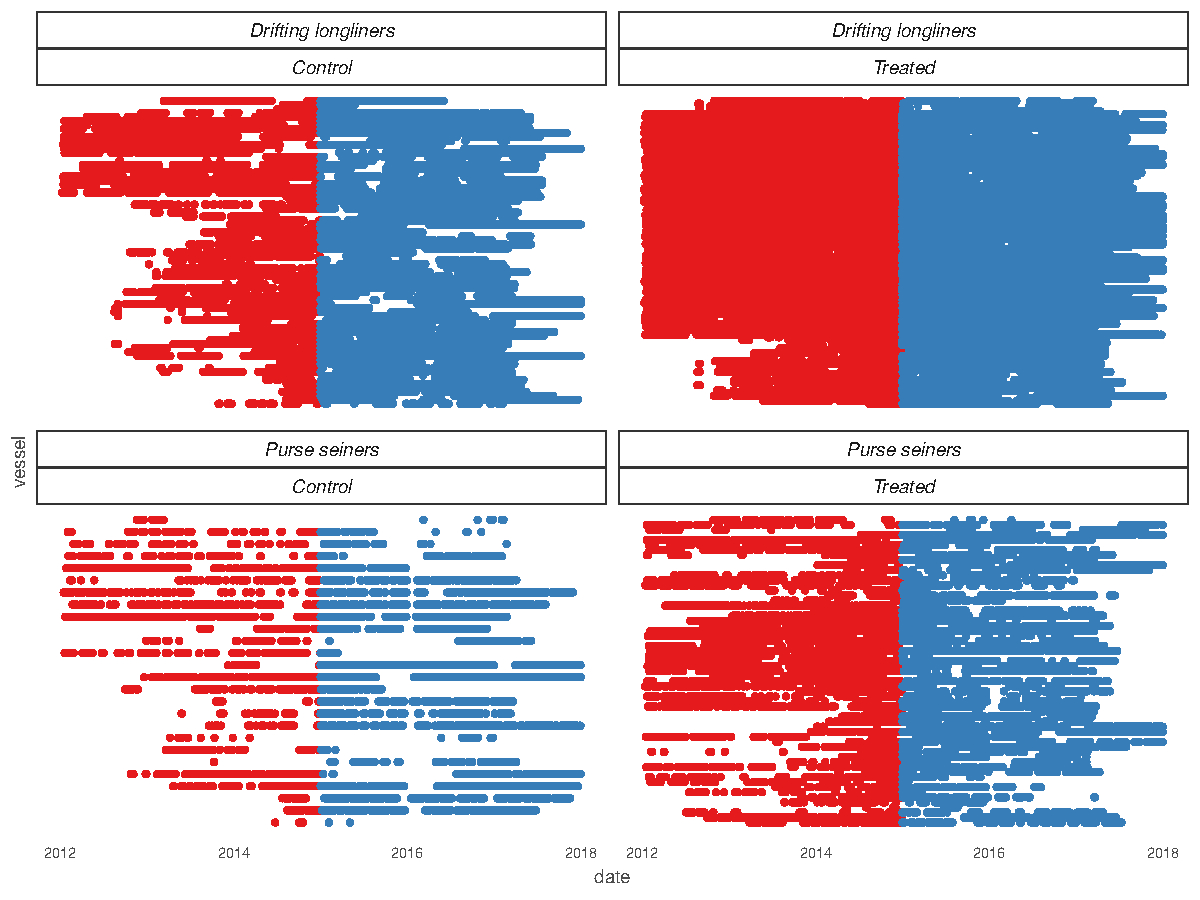
\includegraphics{Manuscript_files/figure-latex/unnamed-chunk-20-1.pdf}
%\caption{\label{fig:unnamed-chunk-20}\label{fig:q1}Interaction of quarters
%and treatment. Control group is all vessels.}
%\end{figure}
%
%\begin{figure}
%\centering
%\includegraphics{Manuscript_files/figure-latex/unnamed-chunk-21-1.pdf}
%\caption{\label{fig:unnamed-chunk-21}\label{fig:q2}Interaction of quarters
%and treatment. Control group is vessels from PNA.}
%\end{figure}
%
%\begin{figure}
%\centering
%\includegraphics{Manuscript_files/figure-latex/unnamed-chunk-22-1.pdf}
%\caption{\label{fig:unnamed-chunk-22}\label{fig:q3}Interaction of quarters
%and treatment. Control group excludes Chinese vessels.}
%\end{figure}
%
%\begin{figure}
%\centering
%\includegraphics{Manuscript_files/figure-latex/unnamed-chunk-23-1.pdf}
%\caption{\label{fig:unnamed-chunk-23}\label{fig:q4}Interaction of quarters
%and treatment. Control group is japanese vessels.}
%\end{figure}
%
%\hypertarget{year-month-did-interactions}{%
%\subsubsection{Year-month DID
%interactions}\label{year-month-did-interactions}}
%
%\begin{figure}
%\centering
%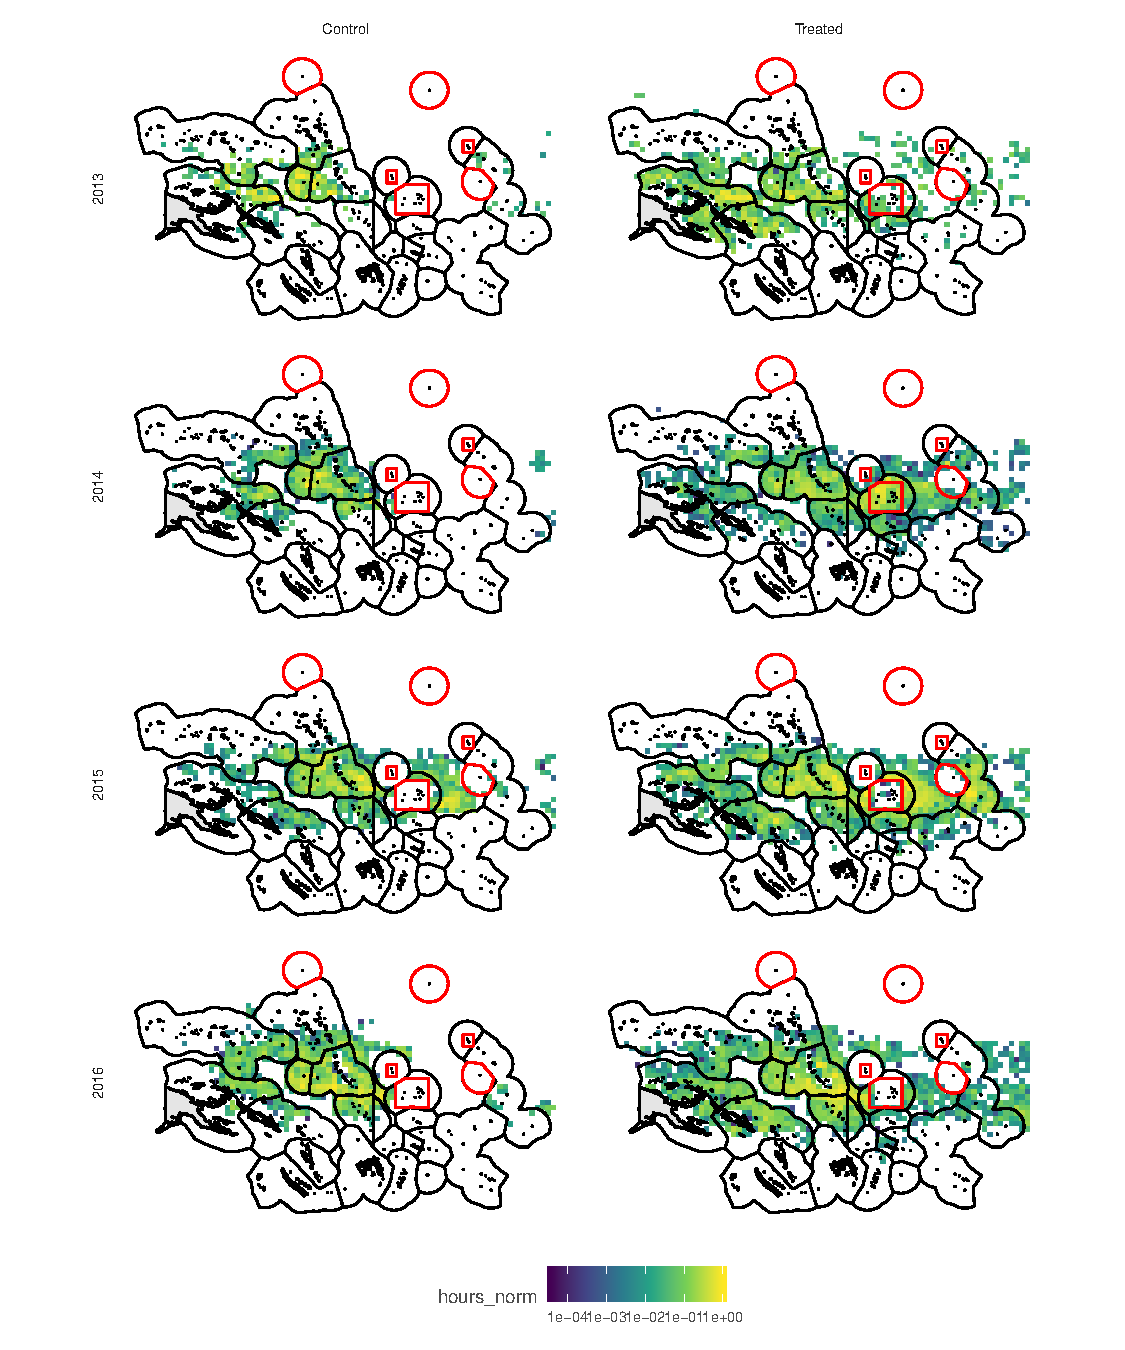
\includegraphics{Manuscript_files/figure-latex/unnamed-chunk-24-1.pdf}
%\caption{\label{fig:unnamed-chunk-24}\label{fig:ym1}Interaction of
%year-month and treatment. Control group is all vessels.}
%\end{figure}
%
%\begin{figure}
%\centering
%\includegraphics{Manuscript_files/figure-latex/unnamed-chunk-25-1.pdf}
%\caption{\label{fig:unnamed-chunk-25}\label{fig:ym2}Interaction of
%year-month and treatment. Control group is vessels from PNA.}
%\end{figure}
%
%\begin{figure}
%\centering
%\includegraphics{Manuscript_files/figure-latex/unnamed-chunk-26-1.pdf}
%\caption{\label{fig:unnamed-chunk-26}\label{fig:ym3}Interaction of
%year-month and treatment. Control group excludes Chinese vessels.}
%\end{figure}
%
%\begin{figure}
%\centering
%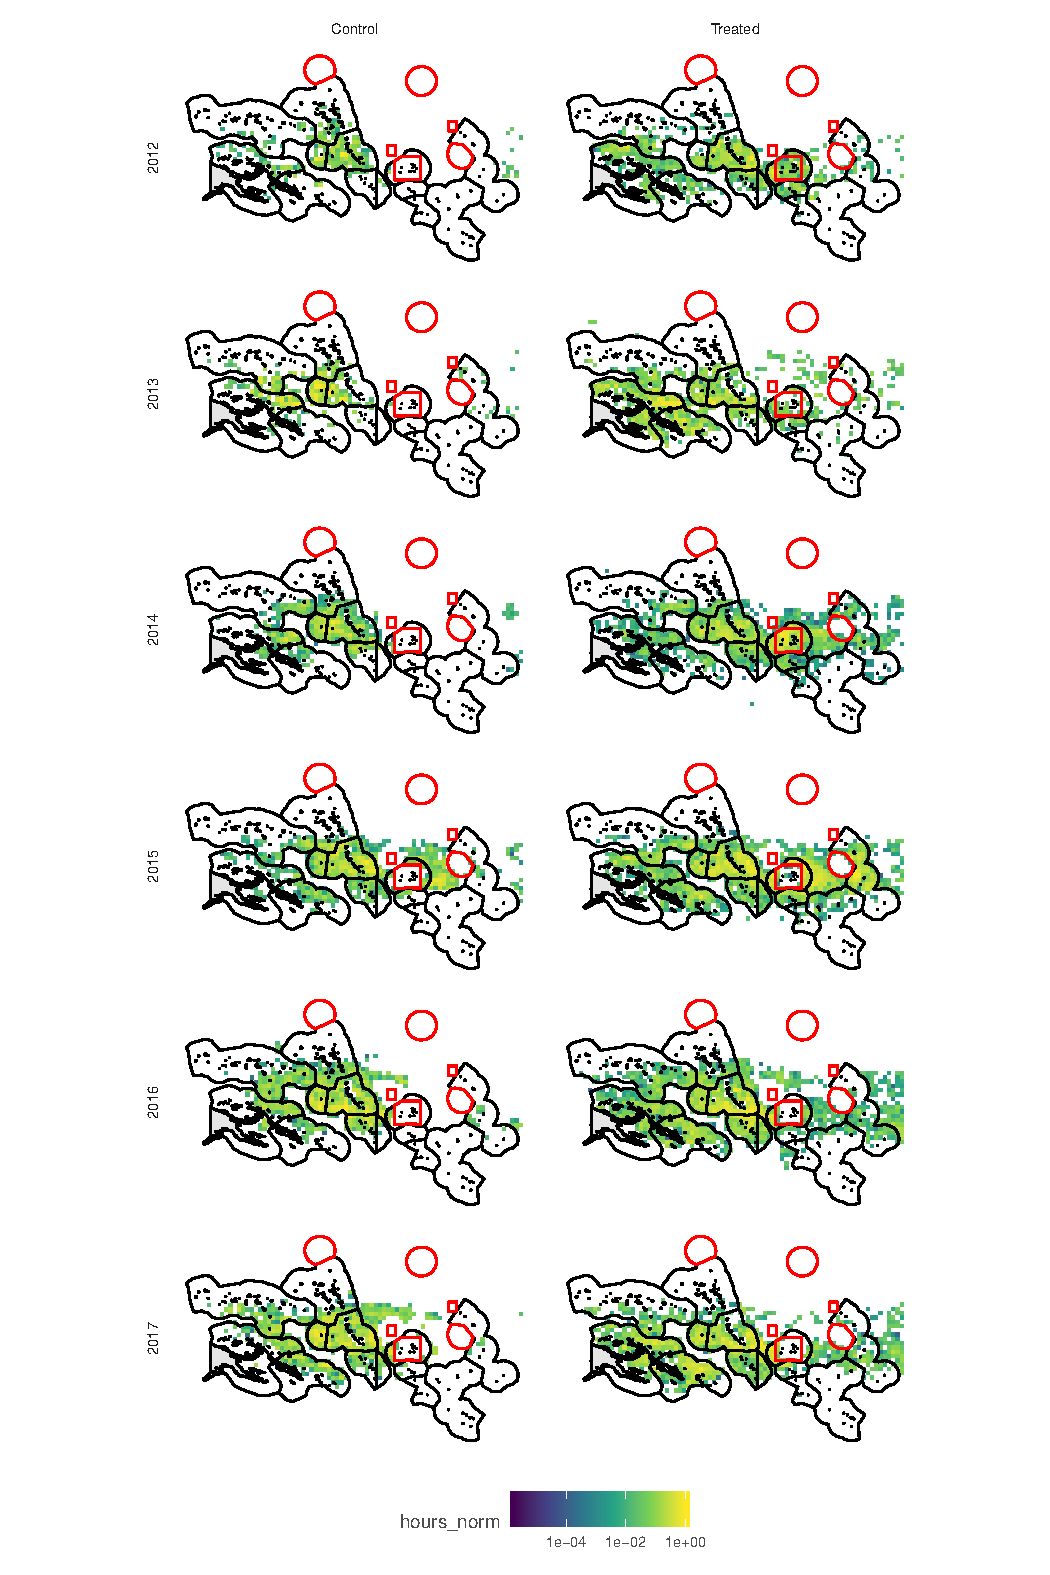
\includegraphics{Manuscript_files/figure-latex/unnamed-chunk-27-1.pdf}
%\caption{\label{fig:unnamed-chunk-27}\label{fig:ym4}Interaction of
%year-month and treatment. Control group is japanese vessels.}
%\end{figure}
%
%\hypertarget{other-measures-of-change-in-behavior}{%
%\subsection{Other measures of change in
%behavior}\label{other-measures-of-change-in-behavior}}
%
%Global Fishing Watch data includes two variables of interest that are
%readily available: distance from shore and distance from port. We use
%these as variables of interest and perform the following regression:
%
%\[
%y = \beta_1Year + \beta_2Treated + \beta_3Year \ Treated + \epsilon
%\]
%
%Where \(y\) is our variable of interest, \(Year\) represent year
%dummies, with 2012 as the reference level, and \(Treated\) indicates
%wether a vessel belongs to the treated or control group.
%
%\clearpage
%
%\hypertarget{distance-from-shore}{%
%\subsubsection{Distance from shore}\label{distance-from-shore}}
%
%\begin{table}[!htbp] \centering 
%  \caption{\label{tab:dist_shore}Regression results for distance from shore. Numbers in parentheses are heteroskedastic-robust standard errors.} 
%  \label{} 
%\begin{tabular}{@{\extracolsep{5pt}}lc} 
%\\[-1.8ex]\hline 
%\hline \\[-1.8ex] 
% & \multicolumn{1}{c}{\textit{Dependent variable:}} \\ 
%\cline{2-2} 
%\\[-1.8ex] & distance\_from\_shore \\ 
%\hline \\[-1.8ex] 
% Constant & 233,057.900$^{***}$ \\ 
%  & (1,558.294) \\ 
%  & \\ 
% year\_c2013 & $-$818.044 \\ 
%  & (2,623.263) \\ 
%  & \\ 
% year\_c2014 & 14,220.260$^{***}$ \\ 
%  & (1,701.637) \\ 
%  & \\ 
% year\_c2015 & 140,980.200$^{***}$ \\ 
%  & (1,668.140) \\ 
%  & \\ 
% year\_c2016 & 32,557.750$^{***}$ \\ 
%  & (1,584.182) \\ 
%  & \\ 
% year\_c2017 & 168,283.100$^{***}$ \\ 
%  & (1,653.912) \\ 
%  & \\ 
% treated & $-$11,371.280$^{***}$ \\ 
%  & (1,688.879) \\ 
%  & \\ 
% year\_c2013:treated & 62,899.900$^{***}$ \\ 
%  & (3,274.205) \\ 
%  & \\ 
% year\_c2014:treated & $-$17,499.020$^{***}$ \\ 
%  & (1,834.090) \\ 
%  & \\ 
% year\_c2015:treated & $-$34,356.840$^{***}$ \\ 
%  & (1,821.587) \\ 
%  & \\ 
% year\_c2016:treated & 72,512.980$^{***}$ \\ 
%  & (1,739.976) \\ 
%  & \\ 
% year\_c2017:treated & $-$62,350.120$^{***}$ \\ 
%  & (1,805.322) \\ 
%  & \\ 
%\hline \\[-1.8ex] 
%Observations & 4,937,666 \\ 
%R$^{2}$ & 0.032 \\ 
%Adjusted R$^{2}$ & 0.032 \\ 
%Residual Std. Error & 297,128.600 (df = 4937654) \\ 
%F Statistic & 14,649.360$^{***}$ (df = 11; 4937654) \\ 
%\hline 
%\hline \\[-1.8ex] 
%\textit{Note:}  & \multicolumn{1}{r}{$^{*}$p$<$0.1; $^{**}$p$<$0.05; $^{***}$p$<$0.01} \\ 
%\end{tabular} 
%\end{table}
%
%\clearpage
%
%\hypertarget{distance-from-ports}{%
%\subsubsection{Distance from ports}\label{distance-from-ports}}
%
%\begin{table}[!htbp] \centering 
%  \caption{\label{tab:dist_port}Regression results for distance from shore} 
%  \label{} 
%\begin{tabular}{@{\extracolsep{5pt}}lc} 
%\\[-1.8ex]\hline 
%\hline \\[-1.8ex] 
% & \multicolumn{1}{c}{\textit{Dependent variable:}} \\ 
%\cline{2-2} 
%\\[-1.8ex] & distance\_from\_port \\ 
%\hline \\[-1.8ex] 
% Constant & 362.707$^{***}$ \\ 
%  & (1.971) \\ 
%  & \\ 
% year\_c2013 & 9.082$^{***}$ \\ 
%  & (3.198) \\ 
%  & \\ 
% year\_c2014 & 105.414$^{***}$ \\ 
%  & (2.148) \\ 
%  & \\ 
% year\_c2015 & 357.746$^{***}$ \\ 
%  & (2.113) \\ 
%  & \\ 
% year\_c2016 & 112.441$^{***}$ \\ 
%  & (2.009) \\ 
%  & \\ 
% year\_c2017 & 356.506$^{***}$ \\ 
%  & (2.099) \\ 
%  & \\ 
% treated & 149.653$^{***}$ \\ 
%  & (2.249) \\ 
%  & \\ 
% year\_c2013:treated & 26.366$^{***}$ \\ 
%  & (4.125) \\ 
%  & \\ 
% year\_c2014:treated & 50.808$^{***}$ \\ 
%  & (2.453) \\ 
%  & \\ 
% year\_c2015:treated & $-$151.268$^{***}$ \\ 
%  & (2.422) \\ 
%  & \\ 
% year\_c2016:treated & $-$49.445$^{***}$ \\ 
%  & (2.311) \\ 
%  & \\ 
% year\_c2017:treated & $-$252.334$^{***}$ \\ 
%  & (2.390) \\ 
%  & \\ 
%\hline \\[-1.8ex] 
%Observations & 4,937,666 \\ 
%R$^{2}$ & 0.047 \\ 
%Adjusted R$^{2}$ & 0.047 \\ 
%Residual Std. Error & 391.757 (df = 4937654) \\ 
%F Statistic & 22,351.480$^{***}$ (df = 11; 4937654) \\ 
%\hline 
%\hline \\[-1.8ex] 
%\textit{Note:}  & \multicolumn{1}{r}{$^{*}$p$<$0.1; $^{**}$p$<$0.05; $^{***}$p$<$0.01} \\ 
%\end{tabular} 
%\end{table}
%
%\hypertarget{effort-redistribution}{%
%\subsection{Effort redistribution}\label{effort-redistribution}}
%
%\hypertarget{rasterized-regions}{%
%\subsubsection{Rasterized regions}\label{rasterized-regions}}
%
%\begin{figure}
%\centering
%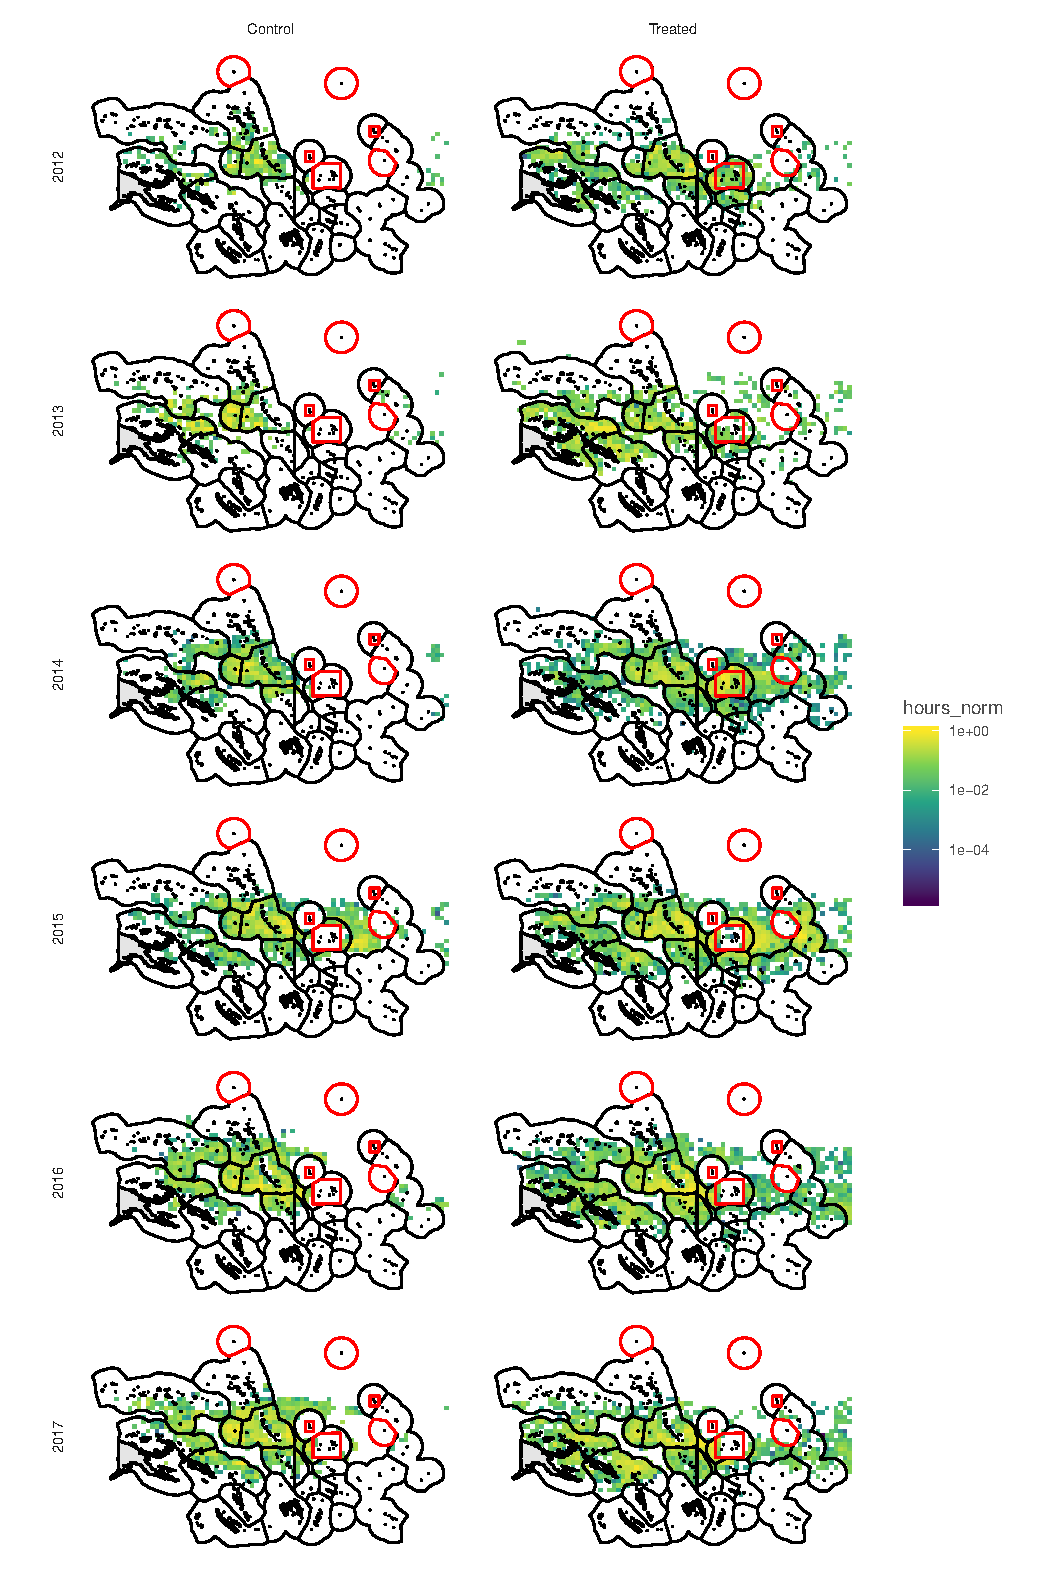
\includegraphics{Manuscript_files/figure-latex/unnamed-chunk-31-1.pdf}
%\caption{\label{fig:unnamed-chunk-31}\label{fig:raster_rgn}Rasterized
%regions. Each color (number) indicates a distinct region.}
%\end{figure}
%
%\hypertarget{fishing-raster}{%
%\subsubsection{Fishing raster}\label{fishing-raster}}
%
%\begin{figure}
%\centering
%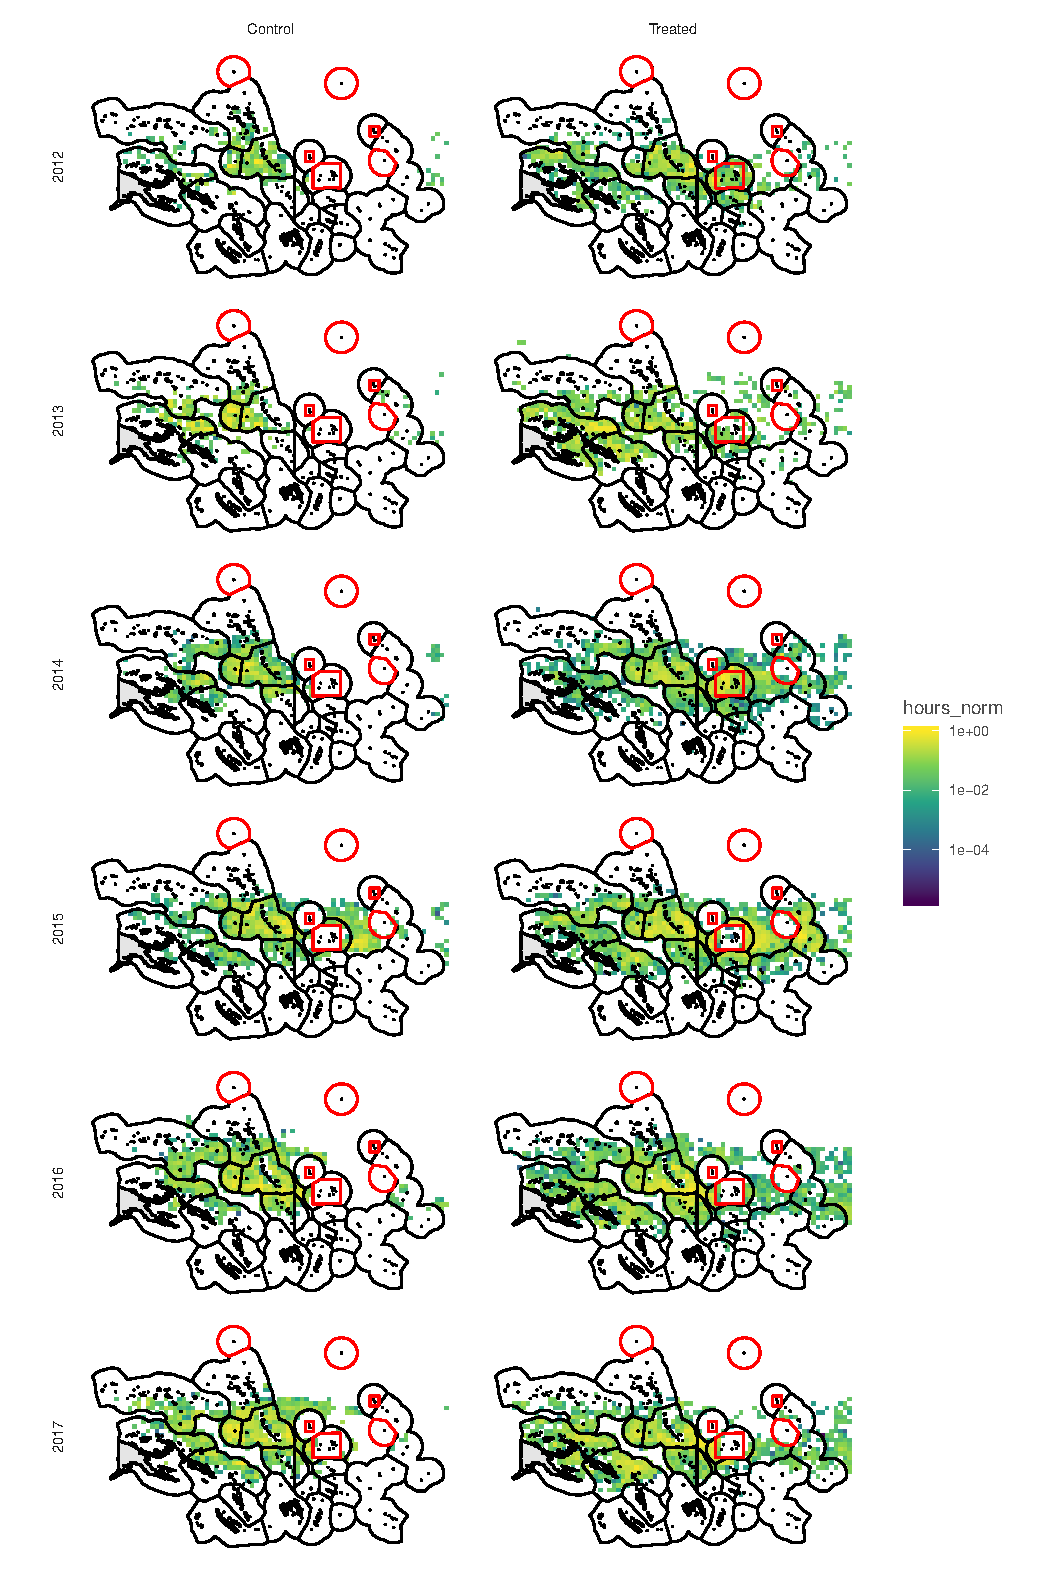
\includegraphics{Manuscript_files/figure-latex/unnamed-chunk-32-1.pdf}
%\caption{\label{fig:unnamed-chunk-32}\label{fig:fishing_raster_full}Yearly
%rasters of fishing hours for each group.}
%\end{figure}
%
%\clearpage


\end{document}
